Statistical analysis was done using the SPSS statistical analysis package v.19 and statistical programming language R version 2.15.1. Statistical significance was evaluated at p=.05. 
\begin{figure}
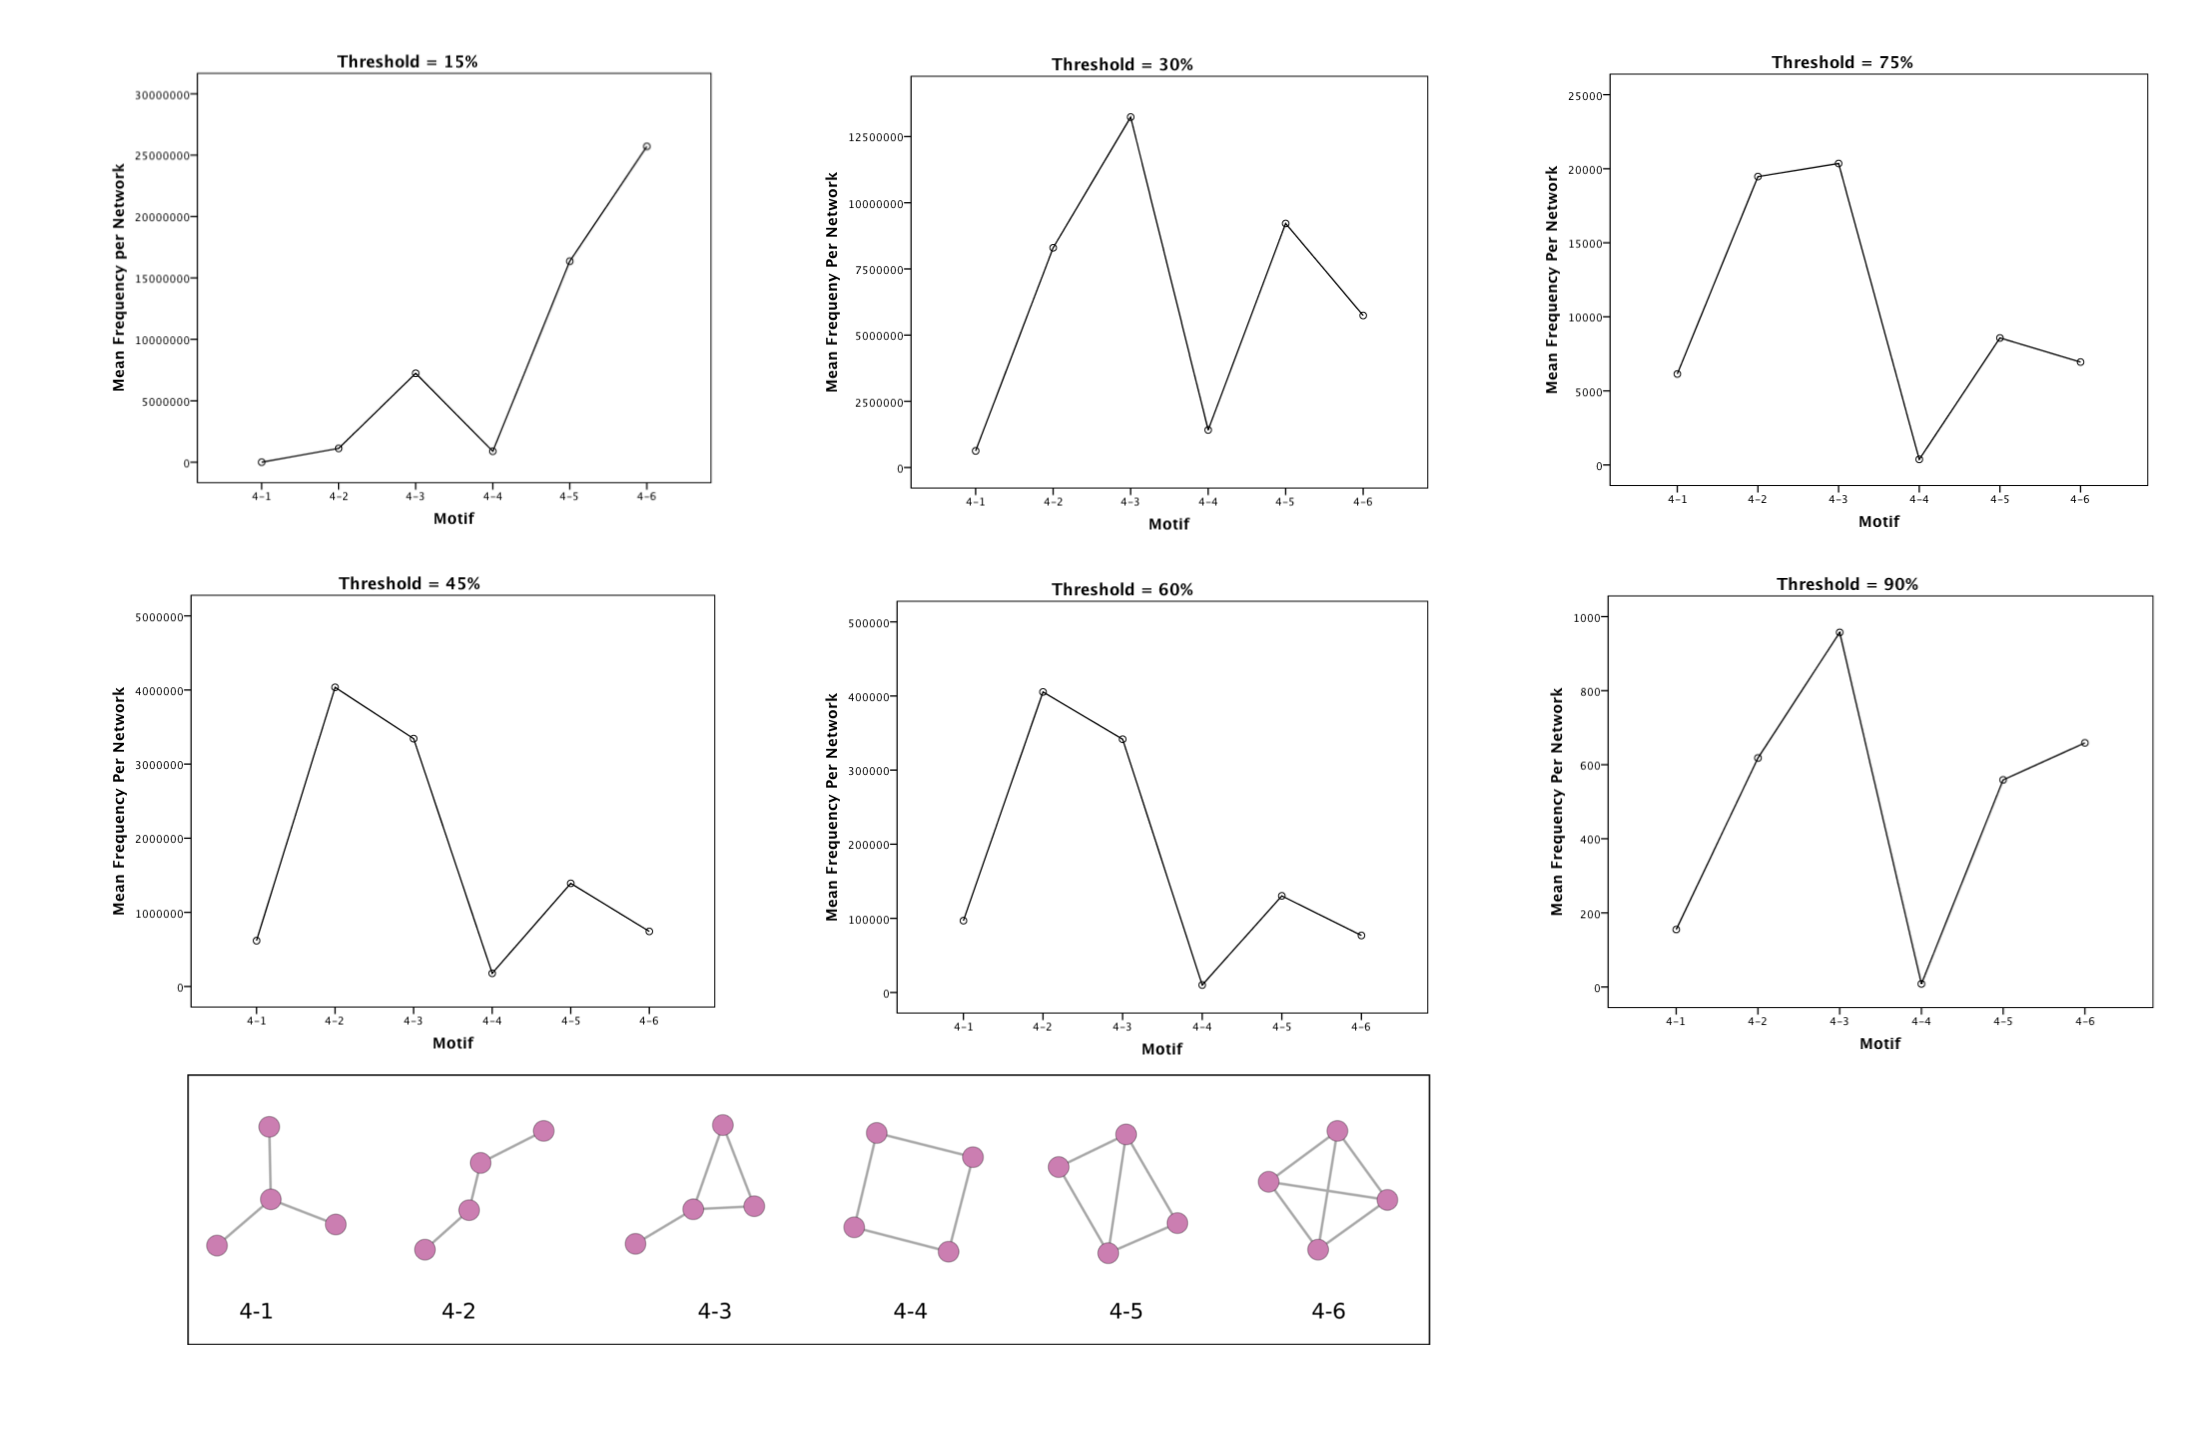
\includegraphics[width=\textwidth,height=\textheight,keepaspectratio]{figs/motif1.png}
\caption{Mean subgraph frequencies by threshold}
\end{figure}

\begin{figure}
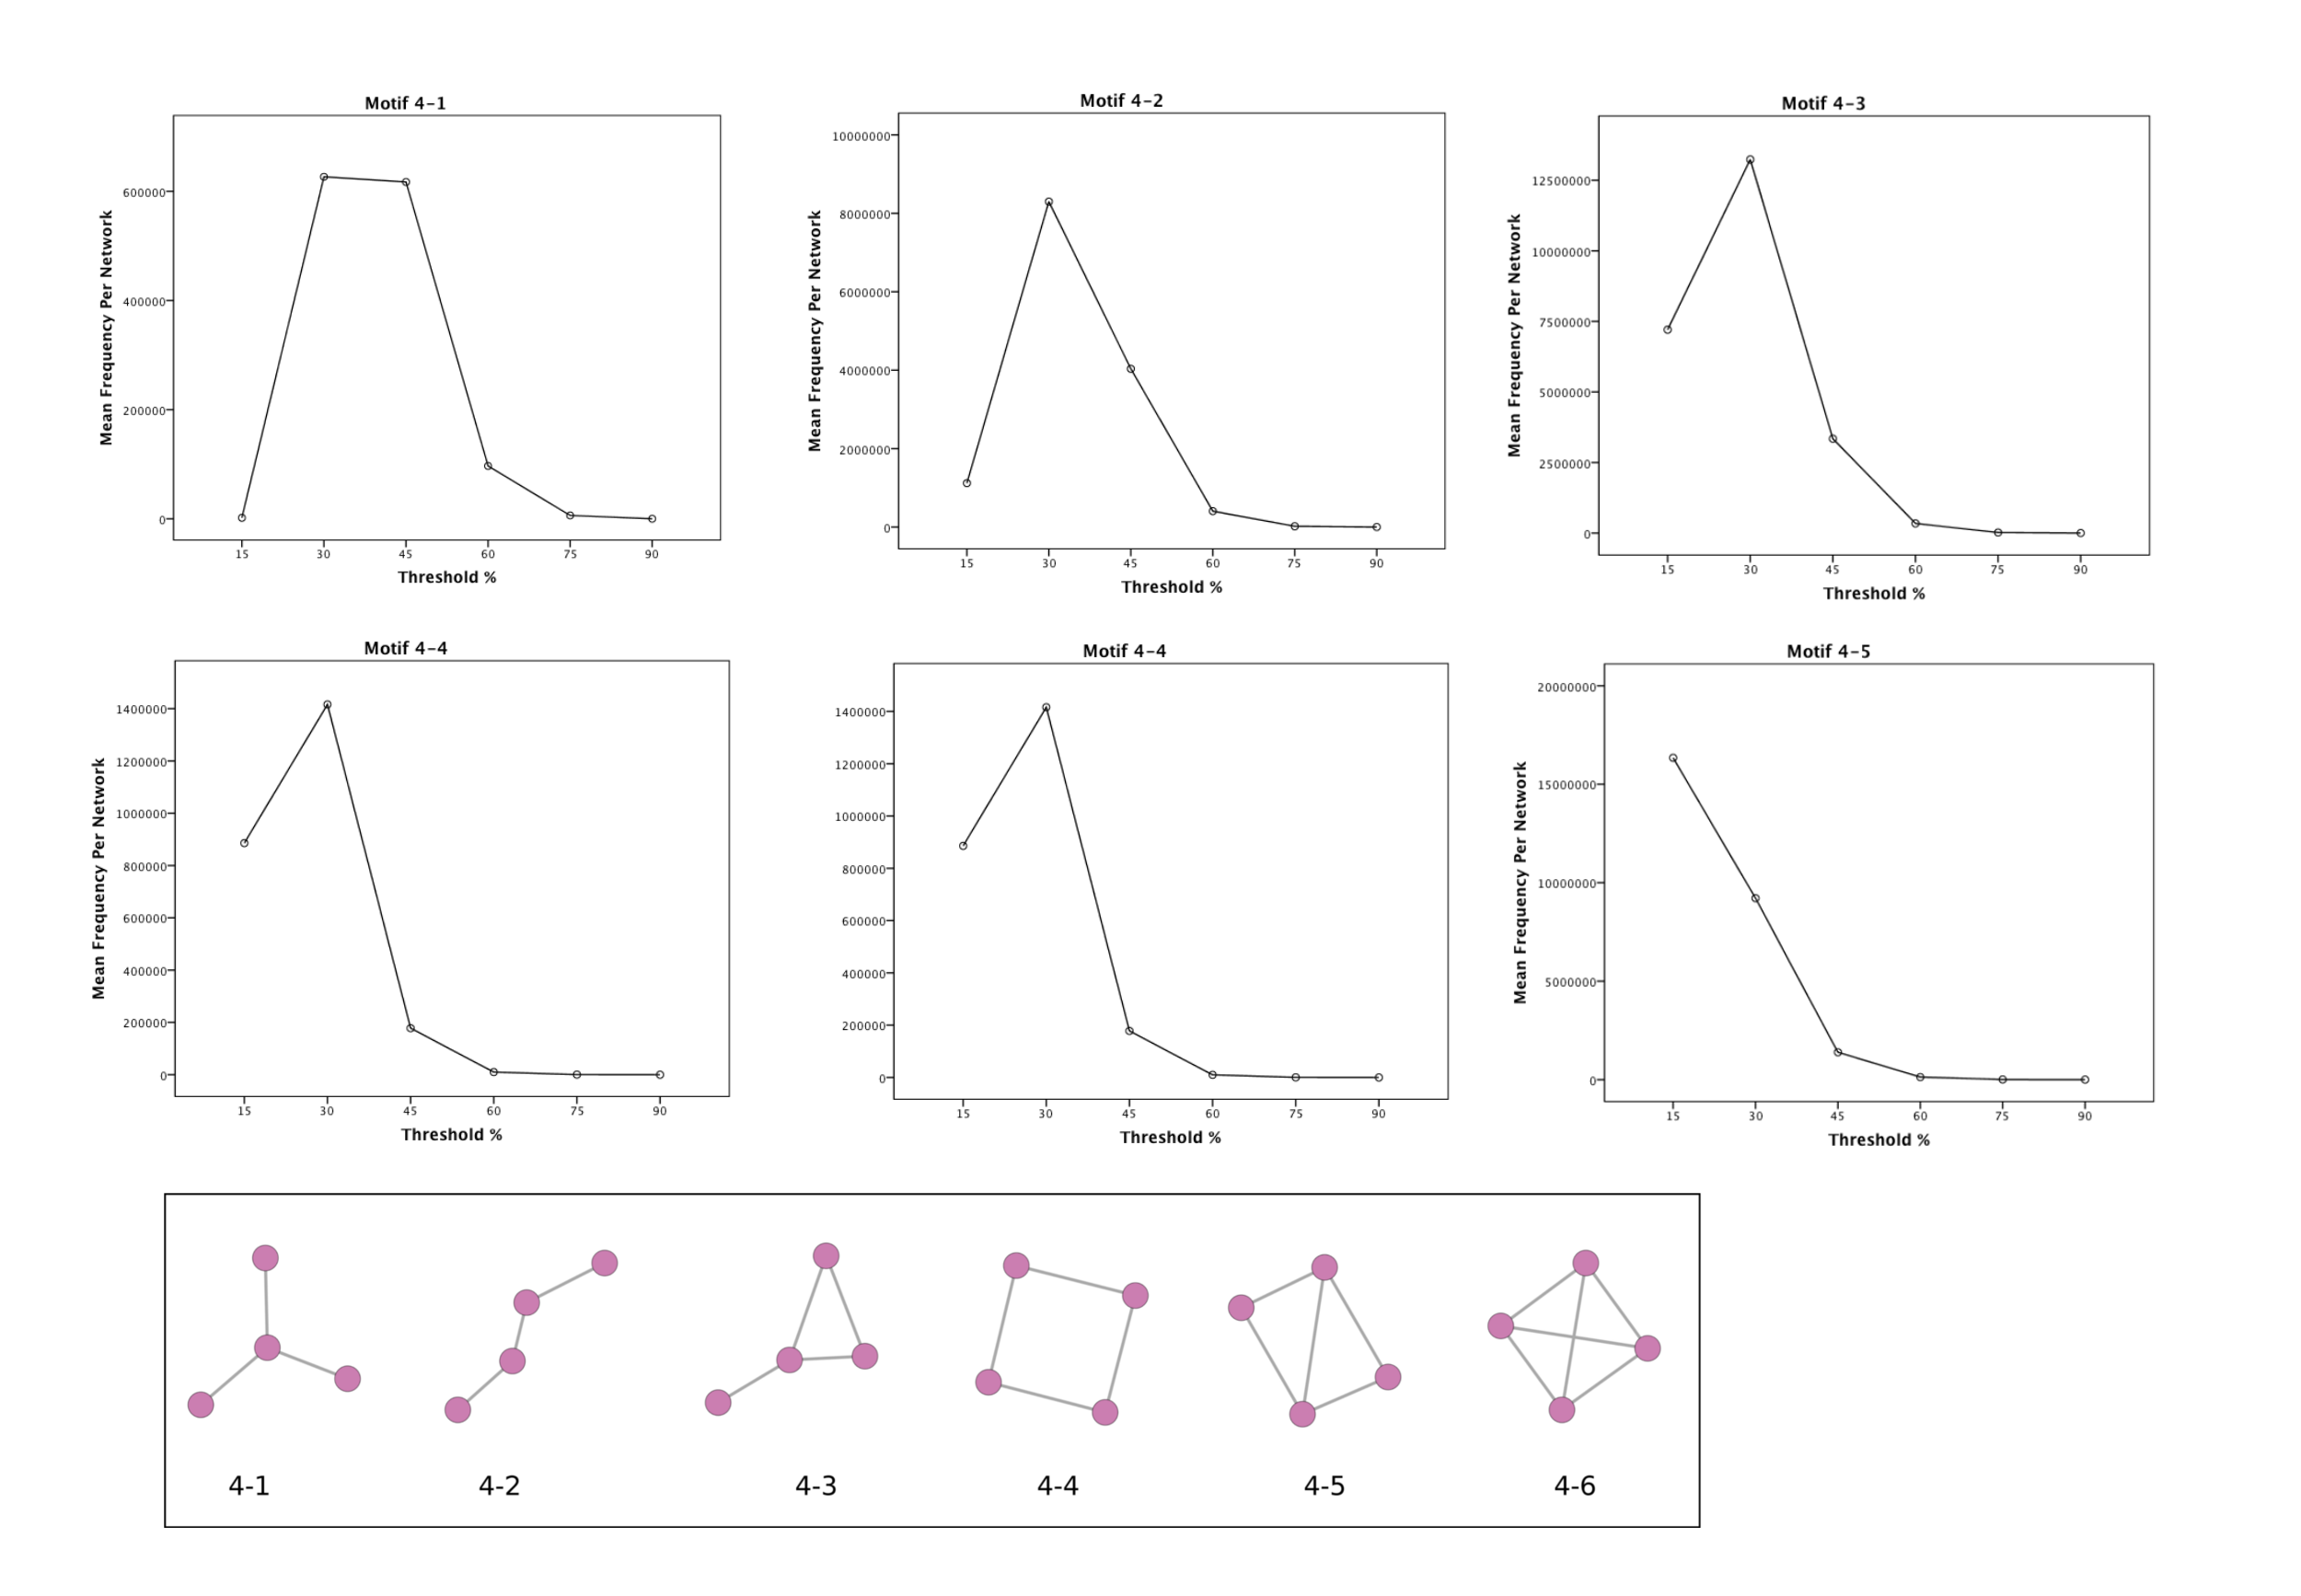
\includegraphics[width=\textwidth,height=\textheight,keepaspectratio]{figs/motif2.png}
\caption{Mean subgraph frequencies by motif}
\end{figure}

\begin{figure}
\caption*{Table 1: Significance Levels for Group Comparisons (ADHD vs. Control) of Mean Frequencies per Network, by Motif and Threshold.}
\begin{center}
\includegraphics{figs/table1.png}
\end{center}
\end{figure}
The 60\% threshold was the only threshold in which significant group differences ($p < .05$) were detected. The 60\% threshold was the most sensitive to group differences between ADHD and control for Motifs 4-2, 4-3, 4-5, and 4-6. Typically developing individuals were found to express less (mean = 394128.5, sd =108528.6) of graph 4-3 than individuals with ADHD (mean = 425151.5, sd = 170217.4, $p < .012$), they also saw less of subgraph 4-3, (mean = 325311.7, sd = 148836.6), (mean = 369994.5, sd = 228788.2, $p < .007$), subgraph 4-5 (mean = 121089.7, sd = 83884.94), (mean = 146333.6, sd = 136222, $p < .009$) and subgraph 4-6 (mean = 64072.93, sd = 73167.64), (mean = 99157.56, sd = 224300.3, $p < .009$). The 90\% threshold was the most sensitive to group differences for Motifs 4-1 and 4-4, however the results were not statistically significant.\\
No signigicant patterns were found across thresholds, however, a more thorough analysis might reveal more.\\
Additionally, an analysis comparing the performance of the GTrieScanner algorithm against the ESU algorithm found that results were not significantly different for most brain network datasets. However, on the C. Elegans neuronal network, GTrieScanner performed at a level more than 10 times greater than the rand-ESU algorithm. Results are shown in 
\begin{figure}
\caption*{Table 2: Comparison of GTrieScanner and Rand-ESU algorithms.}
\includegraphics{figs/gtries-esu.png}
\end{figure}